\documentclass[aspectratio=169]{beamer}
\usepackage{amsmath, tikz, graphicx, cancel}
\usetikzlibrary{arrows, bending}

\newcommand{\bluebox}[1]{\tikz[baseline] \node[fill=blue!20,rectangle,anchor=text]{#1}; }
\newcommand{\boxon}[3]{ \temporal<#2>{\whitebox{$#3$}}{#1{$#3$}}{\whitebox{$#3$}} }
\newcommand{\whitebox}[1]{\tikz[baseline] \node[fill=\bgcolor,rectangle,anchor=text]{#1}; }
\newcommand{\blueboxon}[2]{ \boxon{\bluebox}{#1}{#2} }

\newcommand{\bgcolor}{black!3}
\newcommand{\greyafter}[2]{ \temporal<#1>{}{\textcolor{black}}{\textcolor{black!30}}{#2} }

\setbeamercolor{background canvas}{bg=\bgcolor}

\addtobeamertemplate{frametitle}{\let\insertframetitle\insertsectionhead}{}

\defbeamertemplate{section page}{minimal}[1][]{
  \begin{centering}{}
    \vskip1em\par
    \begin{beamercolorbox}[sep=12pt,center]{part title}
      \usebeamerfont{section title}\insertsection\par
    \end{beamercolorbox}
  \end{centering}
}

\setbeamertemplate{section page}[minimal]
\AtBeginSection{\frame{\sectionpage}}

\title{Lambda Calculus}
\author{Isaac Elliott}

\begin{document}
\beamertemplatenavigationsymbolsempty

% should hand-poll their familiarity with lambda calculus,
% from 'never heard of it' to 'my code is just one giant lambda'
\frame{\titlepage}

\section{What is computation?}

% The theory of computation that we're most commonly exposed to is that
% of state transition systems

\begin{frame}
  \framesubtitle{State-transition systems}
  \frametitle

  \begin{itemize}
    \item<+-> Finite state machines
    \item<+-> Pushdown automata
    \item<+-> Turing machines
  \end{itemize}
\end{frame}

% they all have this idea of a transition function- something that takes
% the current state (plus some other things) as input, and then outputs
% the new state (plus some other things). Then if the computation is to
% continue, the new state becomes the current state, and we start again.
\begin{frame}
  \framesubtitle{State-transition systems}
  \frametitle

  \[ \delta : \; S \times \cdots \; \rightarrow \; S \times \cdots \]
\end{frame}

\begin{frame}
  \framesubtitle{State-transition systems}
  \frametitle

  \begin{columns}
    \begin{column}{0.5 \textwidth}
      \[ \textit{(10)*} \]
      ~ \\
      \[ \Sigma = \{ 0, 1 \} \]
      \[ S = \{ S_0, S_1 \} \]
      ~ \\
      \[ \delta : S \times \Sigma \rightarrow S \]

      \begin{center}
        \begin{tabular}{|c|c c|}
          \hline
          & $0$ & $1$ \\
          \hline
          $S_0$ & $S_2$ & $S_1$ \\
          $S_1$ & $S_0$ & $S_2$ \\
          \hline
        \end{tabular}
      \end{center}

    \end{column}

    \begin{column}{0.5 \textwidth}
      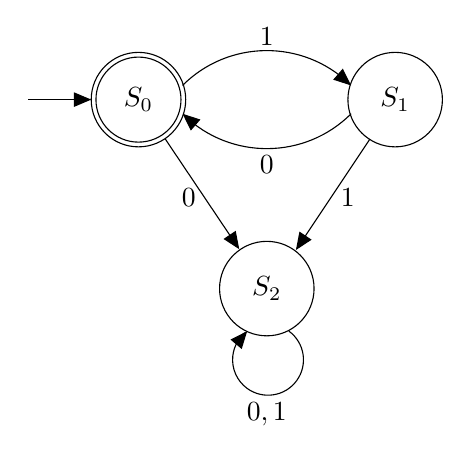
\begin{tikzpicture}[scale=0.2]
        \tikzstyle{every node}+=[inner sep=0pt]
        \draw [arrows=-triangle 45, black] (20.2,-13.9) -- (24.2, -13.9);
        \draw [black] (27.2,-13.9) circle (3);
        \draw [black] (27.2,-13.9) circle (2.7);
        \draw (27.2,-13.9) node {$S_0$};

        \draw [black] (43.5,-13.9) circle (3);
        \draw (43.5,-13.9) node {$S_1$};

        \draw [black] (35.35,-25.9) circle (3);
        \draw (35.35,-25.9) node {$S_2$};

        \draw [arrows=-triangle 45, black] (36.75,-28.6) arc (54:-234:2.25);
        \draw (35.35,-33.1) node [below] {$0,1$};

        \draw [arrows=-triangle 45, black] (28.9, -16.4) -- (33.6, -23.4);
        \draw (30.4, -20.1) node {$0$};

        \draw [arrows=-triangle 45, black] (30.0,-13) to[out=45, in=135] (40.7,-13);
        \draw (35.35,-10.5) node [above] {$1$};

        \draw [arrows=-triangle 45, black] (40.7,-14.8) to[out=225, in=315] (30,-14.8);
        \draw (35.35,-17.4) node [below] {$0$};

        \draw [arrows=-triangle 45, black] (41.9, -16.4) -- (37.2, -23.45);
        \draw (40.5, -20.1) node {$1$};
      \end{tikzpicture}
    \end{column}
  \end{columns}
\end{frame}

\section{$\lambda$-calculus}

\begin{frame}
  \framesubtitle{Definition}
  \frametitle

  \only<1-4>{
  Three expression forms:
  \begin{enumerate}
    \item<2-4> $ \lambda x. \; e $ (abstraction)
    \item<3-4> $ a \; b $ (application - nests to the left - $ a \; b \; c $ is $ (a ; b) \; c $)
    \item<4> $ x $ (variable)
  \end{enumerate}
  }

  \only<5-9>{
  A syntactic operation (substitution)
  \begin{itemize}
    \item<6-9> $ x[x\backslash a] \leadsto a $
    \item<7-9> $ y[x\backslash a] \leadsto y \;\;\; (\text{given} \; y \neq x) $
    \item<8-9> $ (m \; n)[x\backslash a] \leadsto m[x\backslash a] \; n[x\backslash a]$
    \item<9> $ (\lambda y. \; e)[x\backslash a] \leadsto \lambda y. \; e[x\backslash a] \;\;\; (\text{given} \; y \neq x) $
  \end{itemize}
  }

  \only<10-11>{
  A reduction rule (beta reduction)
  \begin{itemize}
    \item<11> $ (\lambda x. e) \; a \leadsto e[x\backslash a] $ 
  \end{itemize}
  }

\end{frame}

\begin{frame}
  \framesubtitle{Terminology}
  \frametitle

  \only<2-8>{
    Bound variable - a variable that has been abstracted over by a lambda \\
    Free variable - a variable that is not bound \\
    \begin{itemize}
      \item<3-8> $ \lambda x. \; x $
      \item<4-8> $ \lambda a. \; \lambda b. \; a \; b $
      \item<5-8> $ \lambda m. \; \lambda n. \; m $
    \end{itemize}
    \onslide<6-8>{Substitution can only affect free variables}
    \begin{itemize}
      \item<7-8> $ x[x \backslash y] \leadsto y $
      \item<8> $ (\lambda x. \; x)[x \backslash y] \leadsto (\lambda x. \; x)$
    \end{itemize}
  }

  \only<9-12>{
    Beta redex - beta red(ucible) ex(pression)
    \begin{itemize}
      \item<10-12> $ (\lambda a. \; a) \; (\lambda b. \; b) $
      \item<11-12> $ (\lambda x. \; \lambda y. \; x) \; a $
      \item<12> $ (\lambda m. \; x) \; b $
    \end{itemize}
  }

  \only<13-16>{
    Value - anything that's not a beta redex
    \begin{itemize}
      \item<14-16> $ a $
      \item<15-16> $ \lambda x. \; x $
      \item<16> $ \lambda a. \lambda b. \; (\lambda x. \; x) \; a $
    \end{itemize}

  }
  \only<17>{
    Evaluate - to reduce to a value
  }
\end{frame}

\begin{frame}
  \framesubtitle{Examples}
  \frametitle

  { \Huge \[ (\lambda x. \; x) \; a \leadsto a \] }
  \[
  \onslide<2->{ \greyafter{2}{ (\lambda x. \; x) \; a } }
  \onslide<3->{ \greyafter{3}{ \; \leadsto x[x \backslash a] } }
  \onslide<4->{ \leadsto a }
  \]
\end{frame}

\begin{frame}
  \framesubtitle{Examples}
  \frametitle

  { \Huge \[ (\lambda x. \; \lambda y. \; x) \; (\lambda b. \; b) \leadsto x \] }
  \[
  \onslide<2->{ \greyafter{2}{ (\lambda f. \; f \; x) \; (\lambda b. \; b) } }
  \onslide<3->{ \greyafter{3}{ \; \leadsto (f \; x)[f \backslash \lambda b. \; b] } }
  \onslide<4->{ \greyafter{4}{ \; \leadsto f[f \backslash \lambda b. \; b] \; x[f \backslash \lambda b. \; b] } }
  \onslide<5->{ \greyafter{5}{ \; \leadsto (\lambda b. \; b) \; x } }
  \onslide<6->{ \greyafter{6}{ \; \leadsto b[b \backslash x] } }
  \onslide<7->{ \leadsto x }
  \]
\end{frame}

\begin{frame}
  \framesubtitle{Currying}
  \frametitle

  \begin{center}
    {
      \renewcommand{\arraystretch}{1.5}
      \begin{tabular}{c|c}
        Maths & $\lambda$-calculus \\
        \hline
        \onslide<2->{$ f(x) = \dots $ & $ f = \lambda x. \; \dots $} \\
        \onslide<3->{$ g(x, y) = \dots $ & $ g = \lambda x. \; \lambda y. \; \dots $} \\
        \onslide<4->{$ g(a, b) $ & $ g \; a \; b $}
      \end{tabular}
    }
  \end{center}

\end{frame}

\begin{frame}
  \frametitle

  % Do you think there are some Turing machine algorithms that couldn't be
  % expressed? Or maybe vice-versa?
  %
  % Some Turing machine programs never halt. Can we create a lambda calculus
  % expression that never stops reducing?

  How does $\lambda$-calculus compare to Turing machines in terms of computability?

  \begin{itemize}
    % I won't prove it, but I will show you some tools that might make this
    % claim seem plausible
    \item<2-> They are equivalent (Church-Turing thesis)
  \end{itemize}

\end{frame}

\section{Church Encoding}

\begin{frame}
  \framesubtitle{Booleans}
  \frametitle

  % Booleans values come in two flavours: true and false
  %
  % It doesn't matter what we call them, so long as we have two different values
  % that support common operations (negation, conjunction, disjunction, etc.)

  \begin{itemize}
    \item<+-> $\texttt{false} = \lambda x. \; \lambda y. \; x$
    \item<+-> $\texttt{true} = \lambda x. \; \lambda y. \; y$
  \end{itemize}

\end{frame}

\begin{frame}
  \framesubtitle{Booleans}
  \frametitle

  \[ not = \; ? \]

\end{frame}

\begin{frame}
  \framesubtitle{Booleans}
  \frametitle

  % we can't define the function by cases
  {

  \renewcommand\CancelColor{\color{red}}
  \[
  \xcancel{
  not(x) =
  \begin{cases}
    \texttt{true} & \mapsto \texttt{false} \\
    \texttt{false} & \mapsto \texttt{true}
  \end{cases}
  }
  \]

  }

\end{frame}

\begin{frame}
  \framesubtitle{Booleans}
  \frametitle

  \[
  \begin{aligned}
    & \texttt{false} & = \lambda x. \; \lambda y. \; x \\
    & \texttt{true} & = \lambda x. \; \lambda y. \; y
  \end{aligned}
  \]

  \[ not = \only<1>{\; ?} \only<2->{ \lambda b. \; b \; \texttt{true} \; \texttt{false} } \]

\end{frame}

\begin{frame}
  \framesubtitle{Booleans}
  \frametitle

  \begin{center}
    % \temporal<1->{}{\textcolor{black}{$ not \; \texttt{true} $}}{\textcolor{black!20}{$ not \; \texttt{true} $}} \\
    \onslide<1->{ \greyafter{1}{$ not \; \texttt{true} $} } \\
    \onslide<2->{ \greyafter{2}{$ (\lambda b. \; b \; \texttt{true} \; \texttt{false}) \; \texttt{true} $} } \\
    \onslide<3->{ \greyafter{3}{$ (b \; \texttt{true} \; \texttt{false})[b\backslash  \texttt{true}] $} } \\
    \onslide<4->{ \greyafter{4}{$ \texttt{true} \; \texttt{true} \; \texttt{false} $} } \\
    \onslide<5->{ \greyafter{5}{$ (\lambda x. \; \lambda y. \; y) \; \texttt{true} \; \texttt{false} $} } \\
    \onslide<6->{ \greyafter{6}{$ (\lambda y. \; y)[x \backslash \texttt{true}] \; \texttt{false} $} } \\
    \onslide<7->{ \greyafter{7}{$ (\lambda y. \; y) \; \texttt{false} $} } \\
    \onslide<8->{ \greyafter{8}{$ y[y\backslash \texttt{false}] $} } \\
    \onslide<9->{ \greyafter{9}{$ \texttt{false} $} }
  \end{center}

\end{frame}

\begin{frame}
  \framesubtitle{Booleans}
  \frametitle

  \[ and = \only<1>{\; ?} \only<2->{ \lambda a. \; \lambda b. \; a \; \texttt{false} \; b } \]

\end{frame}

\begin{frame}
  \framesubtitle{Booleans}
  \frametitle

  % throughout explaining these functions, I kept saying "if a is blah then ..."
  %
  % how would we write if then else?

  \[ ifThenElse = \only<1>{\; ?} \only<2->{ \lambda b. \; \lambda x. \; \lambda y. \; b \; y \; x } \]

\end{frame}

\begin{frame}
  \framesubtitle{Booleans}
  \frametitle

  Booleans embody \textit{choice}

\end{frame}

\begin{frame}
  \framesubtitle{Pairs}
  \frametitle

  \[ \texttt{pair} = \lambda a. \; \lambda b. \; \lambda f. \; f \; a \; b \]
  \[ \texttt{fst} = \lambda p. \; p \; (\lambda x. \; \lambda y. \; x) \]
  \[ \texttt{snd} = \lambda p. \; p \; (\lambda x. \; \lambda y. \; y) \]

\end{frame}

\begin{frame}
  \framesubtitle{Pairs}
  \frametitle

  \[ \texttt{fst} = \lambda p. \; p \; \texttt{false} \]
  \[ \texttt{snd} = \lambda p. \; p \; \texttt{true} \]

  \begin{center}
  You can \textit{choose} whether you want the first or second element
  \end{center}

\end{frame}

\begin{frame}
  \framesubtitle{Natural numbers}
  \frametitle

  A natural number N is represented by N applications of a some function to some argument
  \begin{itemize}
    \item Zero - $f$ is applied 0 times - $\lambda f. \; \lambda x. \; x$
    \item One - $f$ is applied 1 times - $\lambda f. \; \lambda x. \; f \; x$
    \item Two - $f$ is applied 2 times - $\lambda f. \; \lambda x. \; f \; (f \; x)$
    \item Three - $f$ is applied 3 times - $\lambda f. \; \lambda x. \; f \; (f \; (f \; x))$
    \item \dots
  \end{itemize}

  The essence of a natural number is \textit{iteration}

\end{frame}

\begin{frame}
  \framesubtitle{Natural numbers}
  \frametitle

  \begin{itemize}
    \item $ \texttt{zero} = \lambda f. \; \lambda x. \; x $
    \item $ \texttt{suc} = \lambda n. \; \lambda f. \; \lambda x. \; f \; (n \; f \; x) $
  \end{itemize}

\end{frame}

\begin{frame}
  \framesubtitle{Natural numbers}
  \frametitle

  \[ \texttt{suc} \; \texttt{zero} \]
  \[ (\lambda n. \; \lambda f. \; \lambda x. \; f \; (n \; f \; x)) \; \texttt{zero} \]
  \[ (\lambda f. \; \lambda x. \; f \; (n \; f \; x))[n\backslash  \texttt{zero}] \]
  \[ \lambda f. \; \lambda x. \; f \; (\texttt{zero} \; f \; x) \]

  % and if you don't believe me when I say that zero applied to f and x is the same as
  % just x, I can prove it by doing a beta reduction

\end{frame}

\begin{frame}
  \framesubtitle{Natural numbers}
  \frametitle

  \[ add = \only<1>{\; ?} \onslide<2->{ \lambda m. \; \lambda n. \; \lambda f. \; \lambda x. \; m \; f \; (n \; f \; x) } \]

  \onslide<3->{ \[ mult = \; ? \] }
  \onslide<4->{ \[ exp = \; ? \] }
  \onslide<5->{ \[ pred = \; ? \] }

\end{frame}

\section{Repetition}

\begin{frame}
  \framesubtitle{Omega}
  \frametitle

  \[ \Omega = (\lambda x. \; x \; x) \; (\lambda x. \; x \; x) \]

\end{frame}

\begin{frame}
  \framesubtitle{The Y-combinator}
  \frametitle

  \[ Y = \lambda f. \; (\lambda x. \; f \; (x \; x)) \; (\lambda x. \; f \; (x \; x)) \]

\end{frame}

\begin{frame}
  \framesubtitle{Ackermann function}
  \frametitle

  \only<1>{
  \[
  A(m, n) =
  \begin{cases}
    m = 0 & \mapsto n+1 \\
    m > 0, n = 0 & \mapsto A(m-1, 1) \\
    m > 0, n > 0 & \mapsto A(m-1, A(m, n-1)) \\
  \end{cases}
  \]
  }

  \only<2>{
  \[ pred = \dots \]

  \[ is0 = \lambda n. \; n \; (\lambda x. \; \texttt{false}) \; \texttt{true} \]
  }

  \only<3>{
  \[
  \begin{aligned}
  A & = & \\
  & Y & (\lambda f. \; \lambda m. \; \lambda n. \span \\
  & ~ & is0 &\; m  & \\
  & ~ & ~   & (is0 \; n \\
  & ~ & ~   & ~~~  (f \; (pred \; m) \; (f \; m \; (pred \; n))) \span \\
  & ~ & ~   & ~~~  (f \; (pred \; m) \; (\texttt{suc} \; \texttt{zero}))) \span \\
  & ~ & ~   & (\texttt{suc} \; n)) \span
  \end{aligned}
  \]
  }

\end{frame}

\section{Combinator Calculus}

\begin{frame}
  \frametitle

  Four expression forms:
  \begin{itemize}
    \item<2-> $ a \; b $ (application - nests to the left)
    \item<3-> $ \texttt{S} $ (\textbf{S}ubsitution)
    \item<4-> $ \texttt{K} $ (\textbf{K}onstant)
    \item<5-> $ \texttt{I} $ (\textbf{I}dentity)
  \end{itemize}
\end{frame}

\begin{frame}
  \frametitle

  Three reduction rules:
  \begin{itemize}
    \item<2-> $ \texttt{S} \; a \; b \; c \leadsto a \; c \; (b \; c) $
    \item<3-> $ \texttt{K} \; a \; b \leadsto a $
    \item<4-> $ \texttt{I} \; a \leadsto a $
  \end{itemize}

\end{frame}

\begin{frame}
  \frametitle

  \begin{itemize}
    \item Equivalent to $\lambda$-calculus, but without variable binding
    \item $\lambda \rightarrow \texttt{SKI}$
      \begin{itemize}
        \item $ \texttt{S} \rightarrow \lambda a. \; \lambda b. \; \lambda c. \; a \; c \; (b \; c) $
        \item $ \texttt{K} \rightarrow \lambda a. \; \lambda b. \; a $
        \item $ \texttt{I} \rightarrow \lambda a. \; a $
      \end{itemize}
    \item $\texttt{SKI} \rightarrow \lambda$
      \begin{itemize}
        \item ???
        \item Used to compile efficient $\lambda$ programs
        \item \texttt{SKI} is like `machine code' for $\lambda$
      \end{itemize}
  \end{itemize}

\end{frame}

\section{Practical $\lambda$?}

\begin{frame}
  \frametitle

  Is $\lambda$-calculus only a theoretical tool?

  \begin{itemize}
    \item<2-> No!
    \item<3-> Anonymous functions
    \item<4-> Functional programming languages
      \begin{itemize}
        \item Haskell
        \item PureScipt
        \item Elm
      \end{itemize}
  \end{itemize}
\end{frame}

\end{document}
